\chapter{Tổng quan lý thuyết}
\label{Chapter2}

\section{Hệ thống Federated Learning}

\subsection{Định nghĩa}

\textbf{Định nghĩa về FL} \cite{yang2019federated}: Giả sử có $n$ máy khách, máy khách thứ $i$ ký hiệu là $c_i$ $(i\in [1, n])$, chứa tập dữ liệu $D_i$. FL là một quá trình học mà ở đó, các chủ sở hữu dữ liệu (ở đây có thể hiểu là các thiết bị biên) cùng hợp tác huấn luyện một mô hình $\mathcal{M}$ và đạt được độ chính xác $f$ nhưng không có bất kỳ chủ sở hữu dữ liệu $c_i$ nào chia sẻ tập dữ liệu $\mathcal{D}_i$ của chúng.

Gọi $\bar{\mathcal{M}}$ là mô hình máy học được huấn luyện trên tập dữ liệu $\mathcal{D}  = \mathcal{D}_1 \cup \mathcal{D}_2 \cup ... \cup \mathcal{D}_n$ và cho độ chính xác $\bar{f}$. $f$ và $\bar{f}$ chỉ được phép chênh lệch nhau một khoảng nhỏ. Gọi $\delta$ là một giá trị thực không âm, nếu $\mid f-\bar{f}\mid < \delta$ ta nói mô hình $\mathcal{M}$ có \textit{$\delta$ - accuracy loss}.

\textbf{Định nghĩa về tính hợp lệ} \cite{li2021survey}: Ký hiệu $\mathcal{M}_i$ là mô hình được huấn luyện trên tập dữ liệu $\mathcal{D}_i$ và cho độ chính xác $f_i$. Mô hình $\mathcal{M}$ được gọi là hợp lệ nếu tồn tại $i\in [1,n]$ sao cho $f>f_i$.

\subsection{Một hệ thống Federated Learning điển hình}

\textbf{Thành phần và các tương tác trong hệ thống.} Một hệ thống FL (Hình \ref{fig:fl}) thường bao gồm hai thành phần chính: máy chủ (đóng vai trò là đối tượng duy trì mô hình toàn cục) và máy khách (đóng vai trò là đối tượng nắm giữ dữ liệu huấn luyện). Hai thành phần này tương tác với nhau theo ba bước sau \cite{lim2020federated}:

\begin{itemize}
    \item \textit{Khởi tạo.} Máy chủ khởi tạo trọng số $w_G^0$ cho mô hình toàn cục và các siêu tham số cho quá trình huấn luyện. Thông tin này sau đó được gửi đến một tập hợp con các máy khách được chọn để tiến hành huấn luyện.

    \item \textit{Huấn luyện và cập nhật mô hình cục bộ.} Tại bước huấn luyện thứ $t$, máy khách $c_i$ nhận trọng số $w_G^t$ từ máy chủ và tiến hành huấn luyện cục bộ trên tập dữ liệu $D_i$. Tham số $\theta_i^{t}$ thu được sau quá trình huấn luyện (có thể là trọng số $w_i^{t}$ hoặc đạo hàm hàm lỗi $g_i$) được máy khách gửi về máy chủ để tổng hợp.

    \item \textit{Tổng hợp và cập nhật mô hình toàn cục.} Máy chủ nhận tham số $\theta_i^{t}$ gửi về từ các máy khách được chọn trước đó, tiến hành tổng hợp $w_G^{t+1}$ - trọng số mới của mô hình toàn cục và gửi trọng số này đến một tập hợp con các máy khách khác để bắt đầu bước huấn luyện toàn cục mới.
\end{itemize}

Máy chủ sẽ lặp lại bước 2 và bước 3 cho đến khi độ lỗi hội tụ hoặc độ chính xác đạt đến một ngưỡng nhất định. Khi quá trình huấn luyện kết thúc, tham số của mô hình toàn cục sẽ được phân phối đến toàn bộ máy khách trong hệ thống.

\begin{figure}[H]
    \begin{center}
        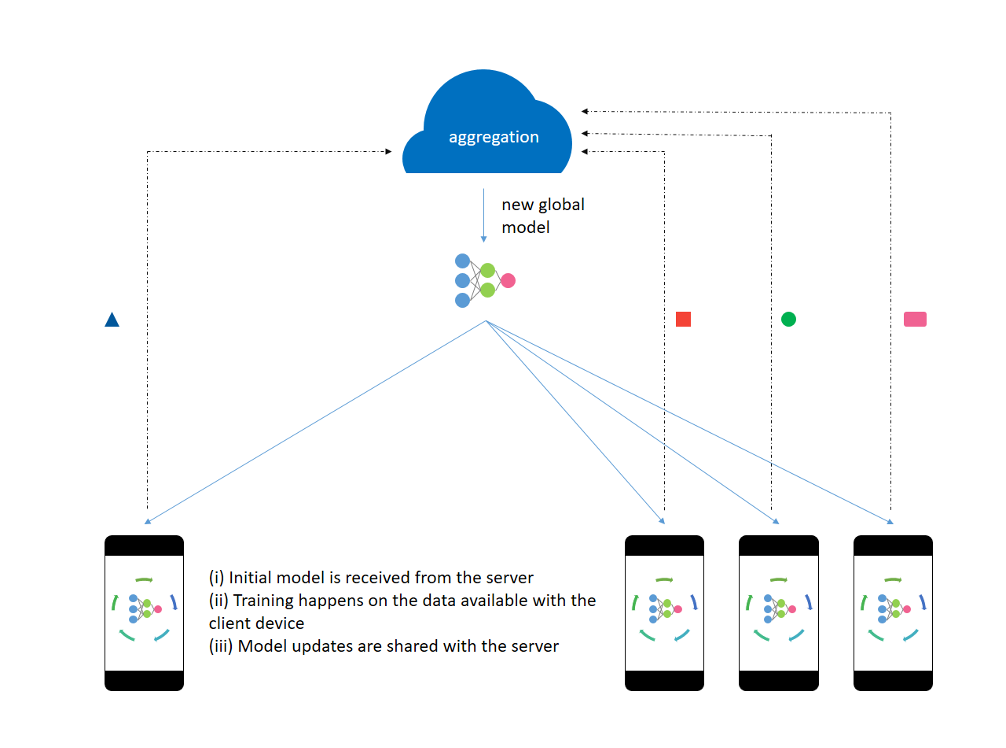
\includegraphics[scale=0.85]{images/fl.png}
        \caption{Hai thành phần chính và quá trình tương tác giữa chúng trong hệ thống FL \cite{chandorikar_2020}}
        \label{fig:fl}
    \end{center}
\end{figure}

\textbf{Mục tiêu của hệ thống FL.} Chúng tôi khảo sát hai mục tiêu của hệ thống FL: (1) - Mục tiêu cục bộ; (2) - Mục tiêu toàn cục.

Các máy khách trong hệ thống hướng đến việc thực hiện mục tiêu cục bộ. Ban đầu, máy khách $c_i$ nhận một trọng số toàn cục $w_G$ từ máy chủ. Máy khách này sau đó sẽ cố gắng tìm kiếm một trọng số $w_i^*$ giúp cực tiểu hóa hàm lỗi cục bộ. Nói cách khác, $w_i^*$ phải thỏa mãn thỏa mãn:

\begin{equation}
    \label{eq:opt_client}
    w_i^* = \arg\min_{w_i}{f_{local}(w_i)}
\end{equation}

Trong đó, $f_{local}(w_i)$ là hàm lỗi trên tập dữ liệu của $c_i$. Với $\alpha$ là siêu tham số học cục bộ, $w_{i(j)}$ là trọng số tại bước huấn luyện $j$ của $c_i$, lời giải của phương trình \ref{eq:opt_client} theo phương pháp SGD có thể được viết như sau:

\begin{equation}
    \begin{cases}
        w_{i(0)} = w_G\\
        w_{i(j)} = w_{i(j-1)} - \alpha \nabla f_{local}(w_{i(j-1)})
    \end{cases}
\end{equation}

Mặt khác, mục tiêu toàn cục, cũng là mục tiêu chính của hệ thống FL, được máy chủ thực hiện bằng cách tìm kiếm một trọng số $w_G^*$ giúp tối thiểu hóa hàm lỗi của cả hệ thống \cite{yin2021comprehensive}:

\begin{dmath}
    \label{eq:opt_server}
    w_G^* = \arg \min_{w_G}{f_{global}(w_G)}
        = \arg \min_{w_G}{\frac{1}{n} \sum_{i=1}^n{f_{local}(w_i)}}
\end{dmath}

Trong đó, $f_{global}(w_G)$ là hàm lỗi toàn cục của hệ thống. Để giải phương trình \ref{eq:opt_server}, máy chủ thực hiện tổng hợp tham số gửi về từ máy khách bằng một trong hai cách: lấy trung bình trọng số \parencite{mcmahan2017communication, aono2017privacy, yoon2021fedmix} hoặc lấy trung bình đạo hàm \parencite{chen2018federated, mcmahan2017learning}.

Đặt $n_i = |\mathcal{D}_i|$ là số điểm dữ liệu của tập $\mathcal{D}_i$, $N = \sum_{i=1}^n{n_i}$ là tổng số điểm dữ liệu có trong cả hệ thống. Phương pháp lấy trung bình trọng số tính toán $w_G^{t+1}$ từ các trọng số của máy khách như sau \cite{mcmahan2017communication}:

\begin{equation}
    w_G^{t+1} = \sum_{i=1}^n{\frac{n_i}{N} w_i^t}
\end{equation}

Trái lại, phương pháp lấy trung bình đạo hàm đòi hỏi máy khách gửi về đạo hàm hàm lỗi sau khi kết thúc quá trình huấn luyện cục bộ. Với $\beta$ là siêu tham số học toàn cục, quá trình tổng hợp được biểu diễn theo công thức:

\begin{dmath}
    w_G^{t+1} = w_G^t - \beta \left[ \frac{1}{n} \sum_{i=1}^n{\frac{n_i}{N} \nabla f_{local}(w_i)} \right]
        = w_G^t - \beta g^t
\end{dmath}

Sau khi khảo sát cả hai phương pháp tổng hợp tham số của máy chủ, nghiên cứu \cite{yin2021comprehensive} chỉ ra rằng, việc lấy trung bình trọng số giúp hệ thống có khả năng chịu được việc mất cập nhật, nhưng không đảm bảo việc hội tụ. Trái lại, việc lấy trung bình đạo hàm giúp hệ thống đảm bảo sự hội tụ nhưng tiêu tốn nhiều chi phí truyền tin hơn. Trong nghiên cứu này, chúng tôi tổng hợp trọng số toàn cục bằng phương pháp lấy trung bình trọng số để phù hợp hơn với giới hạn về chi phí giao tiếp và lưu trữ.

\textbf{Phân loại hệ thống Federated Learning.} Nghiên cứu \cite{yin2021comprehensive} đề xuất các phân loại các hệ thống FL dựa trên phân bố dữ liệu đầu vào của chúng. Theo đó, ba phân bố dữ liệu: (1) - Phân bố dữ liệu theo chiều ngang (Horizontal data partitioning), (2) - Phân bố dữ liệu theo chiều dọc (Vertical data partitioning), (3) - Phân bố dữ liệu hỗn hợp (Hybrid data partitioning) sẽ ứng với ba loại hệ thống FL (Hình \ref{fig:taxonomy_fl}): (1) - Hệ thống FL theo chiều ngang (Horizontal FL), (2) - Hệ thống FL theo chiều dọc (Vertical FL), (3) - Hệ thống học chuyển giao tri thức (Federated Transfer Learning).

\textit{Hệ thống Horizontal FL.} Phân bố dữ liệu theo chiều ngang là kiểu phân bố dữ liệu mà ở đó các bên tham gia vào hệ thống cùng sở hữu các đặc tính dữ liệu giống nhau nhưng giá trị định danh của mẫu dữ liệu của các bên là khác nhau. Ví dụ, khi các bên tham gia hệ thống là các trường đại học, họ sẽ muốn quản lý các thông tin giống nhau về sinh viên như họ và tên, mã số sinh viên,... nhưng không có một sinh viên nào tham gia hai trường đại học cùng một lúc. Kiến trúc Horizontal FL rất phù hợp để huấn luyện mô hình học tuân theo phân phối này \cite{yin2021comprehensive}.

\begin{figure}[H]
    \begin{center}
        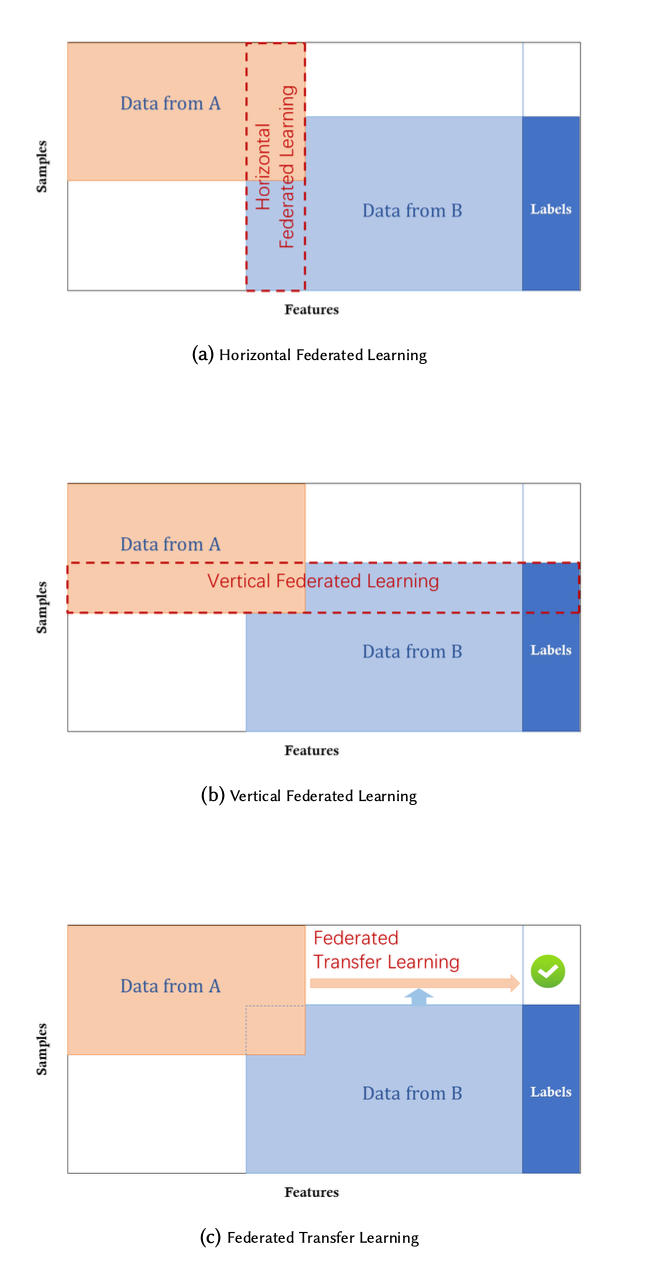
\includegraphics[height=20cm]{images/taxonomy_fl.png}
        \caption{Ba loại hệ thống FL với phân bố dữ liệu tương ứng \cite{yang2019federated}}
        \label{fig:taxonomy_fl}
    \end{center}
\end{figure}

Dựa vào kiến trúc giao tiếp, có thể chia Horizontal FL ra làm hai loại: Kiến trúc client-server và kiến trúc peer-to-peer (P2P). Kiến trúc client-server, hay còn gọi là kiến trúc FL tập trung, về cơ bản sẽ thực hiện các bước huấn luyện giống như đã trình bày trong phần \textbf{Thành phần và các tương tác trong hệ thống}. Trong khi đó, kiến trúc P2P, hay còn gọi là kiến trúc FL phân tán không có một máy chủ cố định. Tại mỗi bước huấn luyện toàn cục, một máy khách trong hệ thống được chọn làm máy chủ. Quá trình huấn luyện sau đó được thực hiện giống như kiến trúc client-server.

Một hệ thống Horizontal FL thường có số lượng máy khách rất lớn, khả năng lưu trữ và tính toán tại các máy khách không cần quá cao (ví dụ như điện thoại thông minh, máy tính bảng) và tần suất một máy khách tham gia huấn luyện là rất thấp.

\textit{Hệ thống Vertical FL.} Đây là kiến trúc phù hợp với phân bố dữ liệu theo chiều dọc. Trong phân bố dữ liệu dạng này, các bên tham gia hệ thống sở hữu các đặc tính dữ liệu khác nhau nhưng giá trị định danh của mẫu dữ liệu của các bên là giống nhau. Ví dụ, khi các bên tham gia hệ thống là ngân hàng và trường đại học. Thuộc tính mà ngân hàng và trường đại học lưu trữ là rất khác nhau nhưng lại chứa thông tin của cùng một người dùng.

\textit{Hệ thống Federated Transfer Learning.} Khi phân bố dữ liệu của các bên tham gia hệ thống không sở hữu chung các đặc tính dữ liệu hay giá trị định danh của từng mẫu, người ta gọi đây là phân bố dữ liệu hỗn hợp. Ví dụ, khi các bên tham gia hệ thống là một ngân hàng ở Hoa Kỳ và một trường đại học ở Việt Nam. Do cản trở địa lý và nhu cầu quản lý thông tin khác nhau, chủ sở hữu dữ liệu này sẽ không có chung thuộc tính hay giá trị định danh nào. Trong trường hợp này, FTL có thể được sử dụng để chuyển giao tri thức giữa các bên tham gia.

Dựa vào các đặc điểm phân loại nêu trên, chúng tôi xếp nghiên cứu của mình vào nhóm hệ thống Horizontal FL tập trung.

\section{Hệ thống Federated Learning trên dữ liệu Non-IID}

Dữ liệu tại các máy khách thường được sinh ra dựa trên nhu cầu của người dùng cuối. Do đó, loại dữ liệu này thường có tính cá nhân hóa cao và không đồng nhất. Nói cách khác, không có bất kỳ phân phối dữ liệu cục bộ nào có thể đại diện cho phân phối trên toàn bộ dữ liệu, phân phối dữ liệu trên hai máy khách khác nhau là khác nhau \cite{zhu2021federated}. Đây chính là ý tưởng mà thuật ngữ \textit{dữ liệu Non-IID} muốn truyền đạt.

Mặt khác, nghiên cứu \cite{zhao2018federated} chỉ ra rằng hệ thống FL có thể bị giảm hiệu quả nghiêm trọng khi đối mặt với dữ liệu Non-IID. Trong phần này, dựa trên nghiên cứu \cite{zhu2021federated} chúng tôi tiến hành khảo sát các kịch bản về dữ liệu Non-IID, các hướng tối ưu hệ thống trên loại dữ liệu này. Trong đó, đi sâu vào hai hướng: Sử dụng Meta Learning và Personalization Layer trong tối ưu hệ thống FL.

\subsection{Các kịch bản Non-IID}



\subsection{Tối ưu hệ thống Federated Learning trên dữ liệu Non-IID}

\textbf{Tối ưu dựa trên dữ liệu.}

\subsubsection{Meta Learning}

\subsubsection{Personalization Layer}
